% Part 1: Detecting DNA-bound RecB molecules
\section*{Results}

\subsection*{Endogenous DNA damage}

\subsubsection*{Imaging RecB molecules}

\begin{figure*}[htbp]
    \centering
    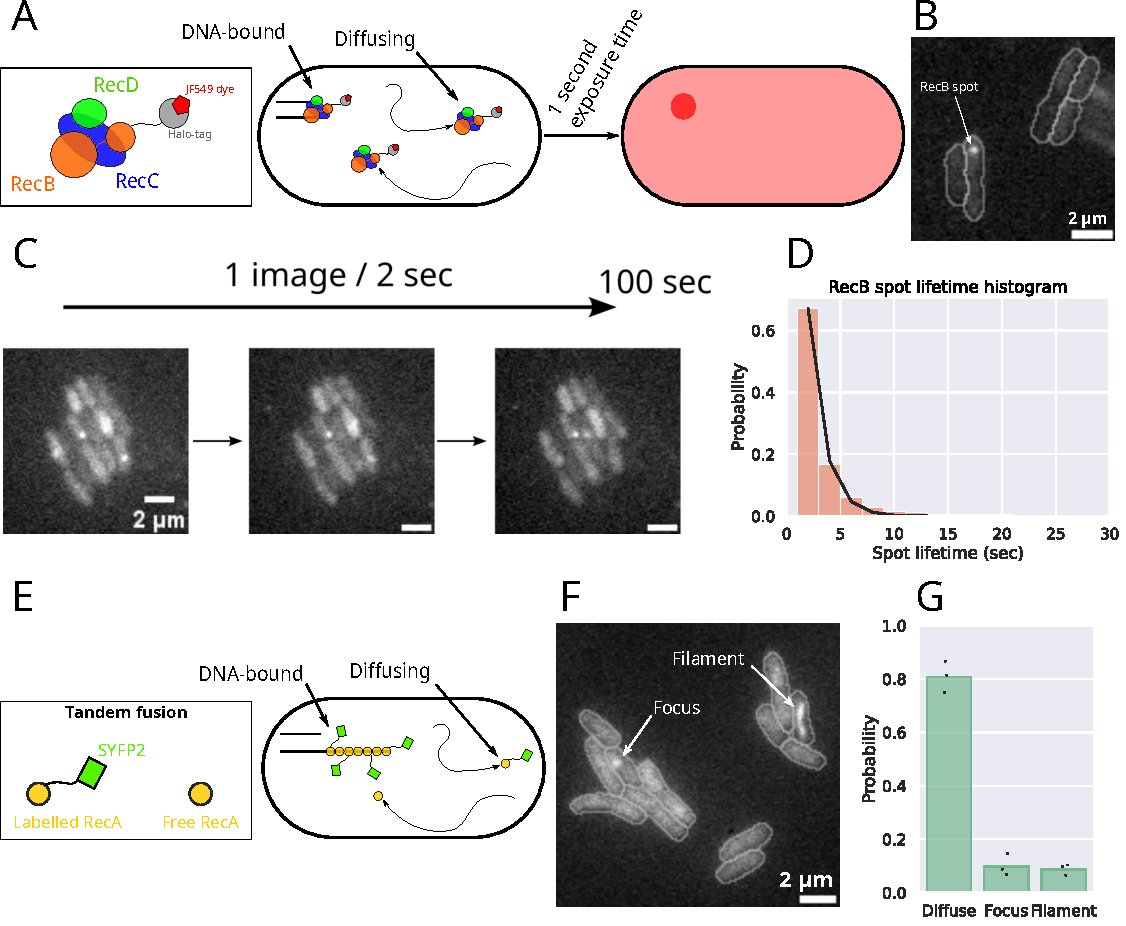
\includegraphics[width=.8\textwidth]{Figures/Fig1_endogenous.pdf}
    \caption{Imaging DSB repair in live \textit{E. coli}. \textbf{(A)} Scheme of our experimental protocol. The RecB subunit of the RecBCD complex is fused to a Halo-tag, bound by the JF549 fluorescent dye. A long exposure time (1 sec) makes diffusing molecules appear as diffuse signal in the cell, while DNA-bound molecules are visible as bright, diffraction-limited spots. \textbf{(B)} Example image of a RecB spot (white arrow). \textbf{(C)} Example images of a timelapse acquisition (1 image every 2 sec for 100 sec). \textbf{(D)} Histogram of the lifetime of RecB spots (bars) fitted with a mono-exponential decay function ($y=a.e^{-k.t}$) \textbf{(E)} Scheme of our RecA imaging system (from \cite{Wiktor2021}). Free and fluorescently labelled RecA are present in equal amounts in the cell. \textbf{(F)} Example image of RecA imaging under endogenous DNA damage. RecA is diffuse in most cells, a RecA focus and a RecA filament are visible in two of the cells (white arrows). \textbf{(G)} Proportions of cells containing the different RecA structures (dots: individual datasets, bars: average between datasets).}
    \label{Fig:endogenous}
\end{figure*}

To image Rec\-BCD in live \textit{E. coli}, we used a Halo-tag fusion to the RecB subunit, conjugated to the JF549 fluorescent dye (Figure \ref{Fig:endogenous}A). The fusion was previously used and characterised in the lab, ensuring specific one-to-one labelling of RecB molecules without adverse effects on the DNA repair process.\cite{Lepore2019a} To detect the binding of RecB to DNA, we applied the previously developed technique of localisation enhancement.\cite{Yu2006, Elf2007}  Since RecB is present at low copy numbers in \textit{E. coli} ($\sim$5 molecules per cell on average\cite{Lepore2019a}), imaging live cells with a long exposure time (1 second) made diffusing molecules appear as weak homogeneous signal in the cell, while DNA-bound molecules formed intense diffraction-limited spots (referred to throughout this article as RecB spots, Figures \ref{Fig:endogenous}B) The complete absence of similar spots in cells expressing the free Halo-tag from a plasmid confirmed that these structures were specific to RecB (Supp. Figure \ref{SIFig:freehalo_image}). Seeing RecB spots in cells that were not exposed to an exogenous source of DNA damage was unsurprising, as these cells are still subject to occasional endogenous DNA damage, such as replication fork collisions which were previously reported to affect $\sim$18\% of cells per cell cycle.\cite{Sinha2018}

Acquiring short timelapse videos (50 images over 100 seconds, Figure \ref{Fig:endogenous}C) allowed us to measure the lifetime of the RecB spots. The resulting histogram was well-fitted by a mono-exponential decay model ($y=a.e^{-k.t}$, with $a$ the fit amplitude and $k$ the dissociation rate from DNA), consistent with a single homogenous population of fluorescent spots (Figure \ref{Fig:endogenous}D). The fitted spot lifetime was 1.5 sec $\pm$ 0.1. This prolonged imaging of the RecB-Halo fusion was only possible thanks to the exceptional photostability of the JF549 dye, which displayed slow photobleaching and no blinking (Supp. Note \ref{note:dye_bleaching} and Supp. Fig. \ref{SIFig:dye_bleaching}).

%% RecA makes foci and filaments
\subsubsection*{RecA forms foci and filaments}
One of RecBCD's purposes when processing a DSB is to facilitate the loading of the RecA protein on single-stranded DNA. To broaden our view of the repair process downstream of RecBCD, we imaged a tandem fusion of RecA with the fluorescent protein SYFP2 (Figure \ref{Fig:endogenous}E).\cite{Wiktor2021} Based on the fluorescence distribution in the cells, we identified three states of RecA: diffuse, forming a bright focus, or forming an elongated filament (Figure \ref{Fig:endogenous}F). Because of the large diversity of shapes observed, especially for RecA filaments, the detection of RecA structures by rule-based algorithms was challenging. Therefore, we designed and trained a deep-learning algorithm capable of classifying individual cells based on the three types of structures cited above (see Methods and Supp. Figure \ref{SIFig:object_class}). This allowed us to quantify the fraction of cells where RecA is freely diffusing to 81\% $\pm$ 6, RecA foci to 10\% $\pm$ 4, and RecA filaments to 9\% $\pm$ 2 (Figure \ref{Fig:endogenous}G). This is consistent with a minority of cells experiencing DNA damage, and being engaged in the repair process.

% Part 2: Separating genuine RecB binding events
\subsection*{Finding DNA binding events}

\begin{figure*}[htbp]
    \centering
    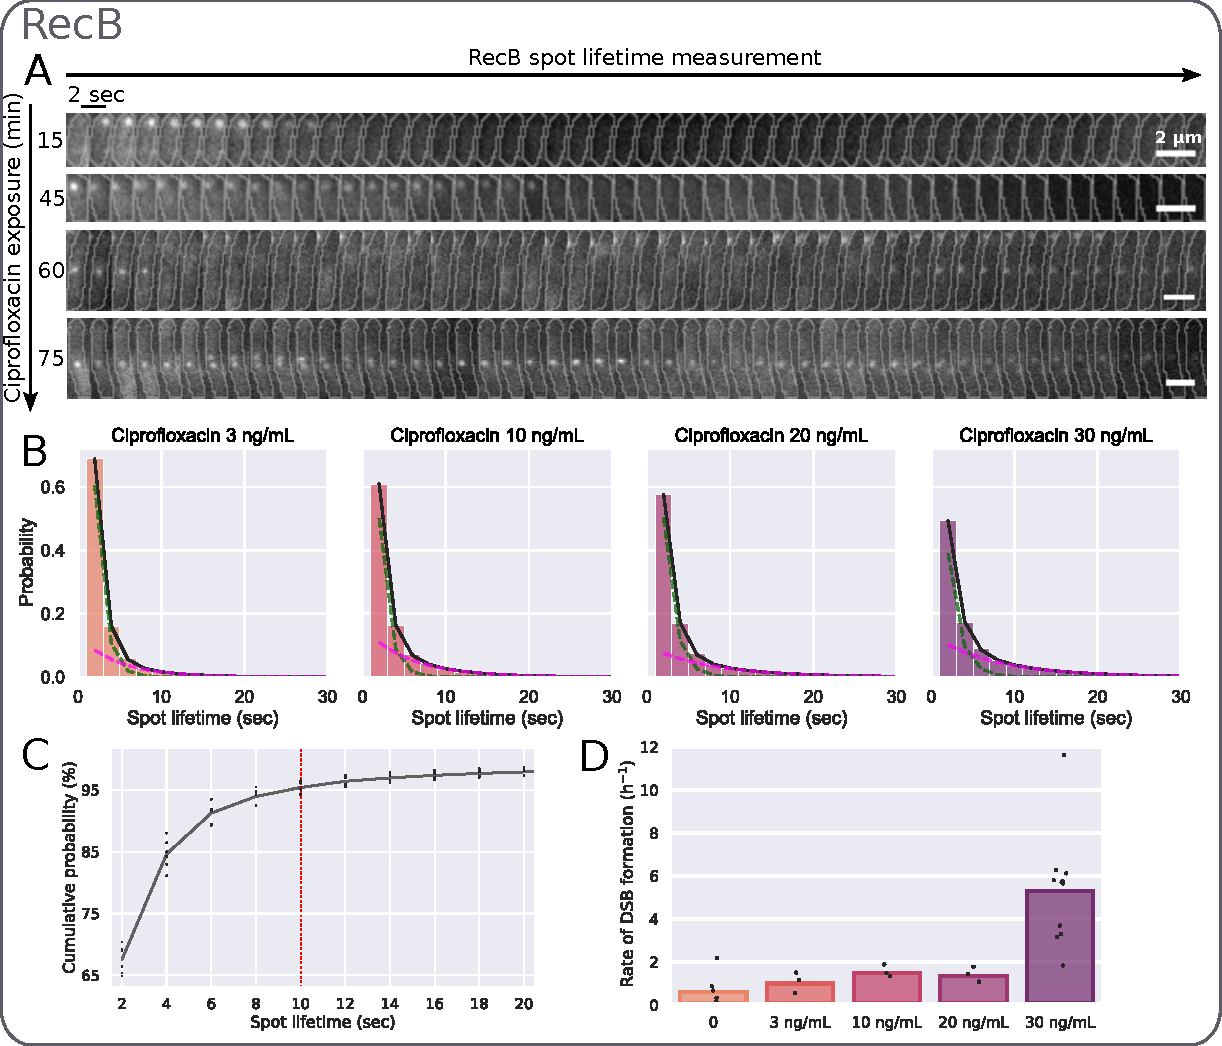
\includegraphics[width=.8\textwidth]{Figures/Fig2_RecB_binding.pdf}
    \caption{RecB DNA binding under ciprofloxacin exposure. \textbf{(A)} Example kymographs of RecB throughout an acquisition. A short timelapse (100 sec) is acquired at a different position every 2 min for 75 min. \textbf{(B)} RecB spot lifetime histograms at 3, 10, 20 and 30 ng/mL ciprofloxacin (bars), fitted with a bi-exponential decay model (black line, fit components showed as dashed lines). \textbf{(C)} Probability of a spot corresponding to a DNA-bound RecB molecule, for cells over-expressing the Gam protein. Black dots show individual datasets, the black line is the average between them, and the red dashed line shows the smallest lifetime at which RecB spots have 95\% probability to be DNA-bound. \textbf{(D)} Recruitment rate of RecB on DNA at different ciprofloxacin concentrations. Black points show individual datasets, and bars the median value.}
    \label{Fig:lifetime_fits}
\end{figure*}

%% We add ciprofloxacin to increase the level of DNA damage
To gain more insight into DNA binding by RecB, we induced additional DSBs by adding the DSB-inducing antibiotic ciprofloxacin to agar pads before imaging. Cells were left to settle down on the pad for 10 min, after which 50-frame timelapse videos were acquired at a rate of one position every 2 min (Figure \ref{Fig:lifetime_fits}A) for 60 min. This allowed us to quantify RecB binding at different time points ranging from 15 to 75 min after the start of ciprofloxacin exposure.

%% RecB spot lifetime histograms change upon exposure to ciprofloxacin
%%% They are not well-fitted by a monoexponential decay (SI fig)
%%% We fit with a bi-exponential decay model
%%% Mention lifetimes/proportions, in table
Upon exposure to ciprofloxacin, the RecB spot lifetime histograms contained more long-lived spots. Fitting with a mono-exponential decay model as in Figure \ref{Fig:endogenous}D did not account well for these long-lived spots (Supp. Figure \ref{SIFig:monoexp_fits}), especially at the higher ciprofloxacin concentrations. This suggested that the new long-lived spots that appeared under exposure to ciprofloxacin corresponded to a new population of RecB spots, that had a slower dissociation rate from DNA than the ones observed under endogenous damage. Indeed, fitting with a bi-exponential decay model ($y = a_1.e^{-k_1.t} + a_2.e^{-k_2.t}$) accounted much better for the longer-lived RecB spots (Figure \ref{Fig:lifetime_fits}B). The bi-exponential fit outlined two populations of spots with different lifetimes: a short-lived one, with lifetimes ranging from 1.4 to 1.7 sec, and a longer-lived one, with lifetimes ranging from 10 to 14 sec (Table \ref{tab:fit_results}). Even though the short-lived spots always represented a majority of events (over 90\% of the spots), the proportion of long-lived spots tended to increase under higher ciprofloxacin exposure (from 1.4\% $\pm$ 0.3 under 3 ng/mL ciprofloxacin to 5.5\% $\pm$ 1.4 under 30 ng/mL ciprofloxacin).

\begin{table}[htbp]
    \centering
    \caption{Parameters derived from the spot lifetime histogram fits (Figures \ref{Fig:endogenous}D and \ref{Fig:lifetime_fits}B). The lifetime was calculated as the inverse of the fitted dissociation rate. Values are given as the median $\pm$ standard deviation over at least 3 independent datasets.}
    \begin{tabular}{llll}
        \toprule
         &  & Lifetime (sec) & Population (\%) \\
        Ciprofloxacin & Type &  &  \\
        \midrule
        \multirow[t]{2}{*}{0} & Short & 1.4 $\pm$ 0.2 & 98.2 $\pm$ 1.0 \\
         & Long & 9.5 $\pm$ 9.7 & 1.8 $\pm$ 1.0 \\
        \cline{1-4}
        \multirow[t]{2}{*}{3 ng/mL} & Short & 1.5 $\pm$ 0.1 & 98.6 $\pm$ 0.3 \\
         & Long & 10.5 $\pm$ 1.3 & 1.4 $\pm$ 0.3 \\
        \cline{1-4}
        \multirow[t]{2}{*}{10 ng/mL} & Short & 1.7 $\pm$ 0.2 & 97.6 $\pm$ 0.6 \\
         & Long & 13.7 $\pm$ 2.3 & 2.4 $\pm$ 0.6 \\
        \cline{1-4}
        \multirow[t]{2}{*}{20 ng/mL} & Short & 1.6 $\pm$ 0.2 & 96.6 $\pm$ 0.8 \\
         & Long & 11.8 $\pm$ 2.1 & 3.4 $\pm$ 0.8 \\
        \cline{1-4}
        \multirow[t]{2}{*}{30 ng/mL} & Short & 1.7 $\pm$ 0.2 & 94.5 $\pm$ 1.4 \\
         & Long & 13.3 $\pm$ 2.2 & 5.5 $\pm$ 1.4 \\
        \cline{1-4}
        \bottomrule
        \end{tabular}
    \label{tab:fit_results}
\end{table}

%% To check what these two populations are, we use the Gam protein to prevent DNA binding and fit with the same model
%%% Short-lived population stays, long-lived one is removed
%%% Interpretation: because of its size, the RecBCD-Halo-Gam complex can sometimes form spots (SI Note + SI Fig), which creates short spots
%%% Therefore, we are unable to assign short DNA binding events, but we can confidently detect longer DNA binding events
To determine whether both short- and long-lived spots resulted from RecB binding to DNA, we measured RecB spot lifetime in the presence and absence of ciprofloxacin while over-expressing the Gam protein of phage $\lambda$ from a plasmid. The Gam protein was previously shown to bind in place of DNA on the RecBCD complex\cite{Wilkinson2016}, and its overexpression is expected to abolish RecBCD binding to DNA. Accordingly, cells that over-expressed Gam and were exposed to high ciprofloxacin (30 ng/mL) showed little elongation compared to cells that did not overexpress Gam (Supp. Figure \ref{SIFig:Gam_cell_length}), indicating that most cells did not induce the SOS response, due to the inability of the RecBCD-Gam complex to bind to DSBs. The resulting RecB spot lifetime histograms showed a near-complete disappearance of the long-lived spots, while short-lived ones were still present (Supp. Figure \ref{SIFig:Gam_RecB_lifetimes_fits}). This was confirmed by fitting the histogram with our bi-exponential decay model, which found proportions of long-lived spots ($\sim$3\%) similar to those in wild-type cells that were not exposed to ciprofloxacin (2.6\%, Table \ref{tab:fit_results}). This confirmed that (i) long-lived RecB spots correspond to RecB molecules that have bound to DNA, and (ii) short-lived RecB spots can result from other causes than short-lived DNA binding (Supp. Note \ref{note:spurious_spots} and Supp. Figure \ref{SIFig:displacement_simul}). Spots that are visible only for a few seconds cannot be reliably assigned to one or the other category. However, based on the Gam overexpression data, we determined that any spot with a lifetime over 10 sec had 95\% probability to be DNA-bound (Figure \ref{Fig:lifetime_fits}C).

%% We use the number of spots and proportion of long-lived spots to estimate the rate of recruitment of RecB on the DNA (Fig 2D)
%% Mention/link to discussion on relationship between RecB recruitment rate and DSB formation rate
Whereas the lifetime of the fluorescent spots informs us on how long RecB stays bound to DNA, the rate of appearance of spots helps us estimate the rate of recruitment of RecB to DSBs under each DNA damage condition (Figure \ref{Fig:lifetime_fits}D). To achieve this, we quantified for each timelapse the total number of spots that belong to the "long-lived" (i.e. RecB bound to DNA) category. Since the short- and long-lived populations cannot be clearly separated from the lifetime histograms (Figure \ref{Fig:lifetime_fits}B), we used an "ensemble-level" approach. For each dataset, we multiplied the total number of spots that appeared during the timelapse by the proportion of long-lived spots retrieved from the lifetime histogram fits, which gave us an estimate of the number of DNA-bound RecB per timelapse, from which a number of recruitment events per hour can be calculated. We estimated that under endogenous damage or low ciprofloxacin concentrations, 1 to 2 RecB molecules are recruited to the DNA per hour on average. This is roughly consistent with the previous estimate of 18\% of cells generating an endogenous DSB per cell cycle\cite{Sinha2018} (see discussion). At ciprofloxacin concentrations above the MIC (30 ng/mL), the recruitment rate increased sharply to an average of 5 RecB recruited per hour. Furthermore, we expect that this recruitment rate gives a close estimate of the rate of formation of DSBs (see discussion).

% Part 3: Effects of DSBs and the repair process on the cell
\subsection*{Ciprofloxacin exposure induces formation of RecA filaments and nucleoid compaction}

\begin{figure*}[htbp]
    \centering
    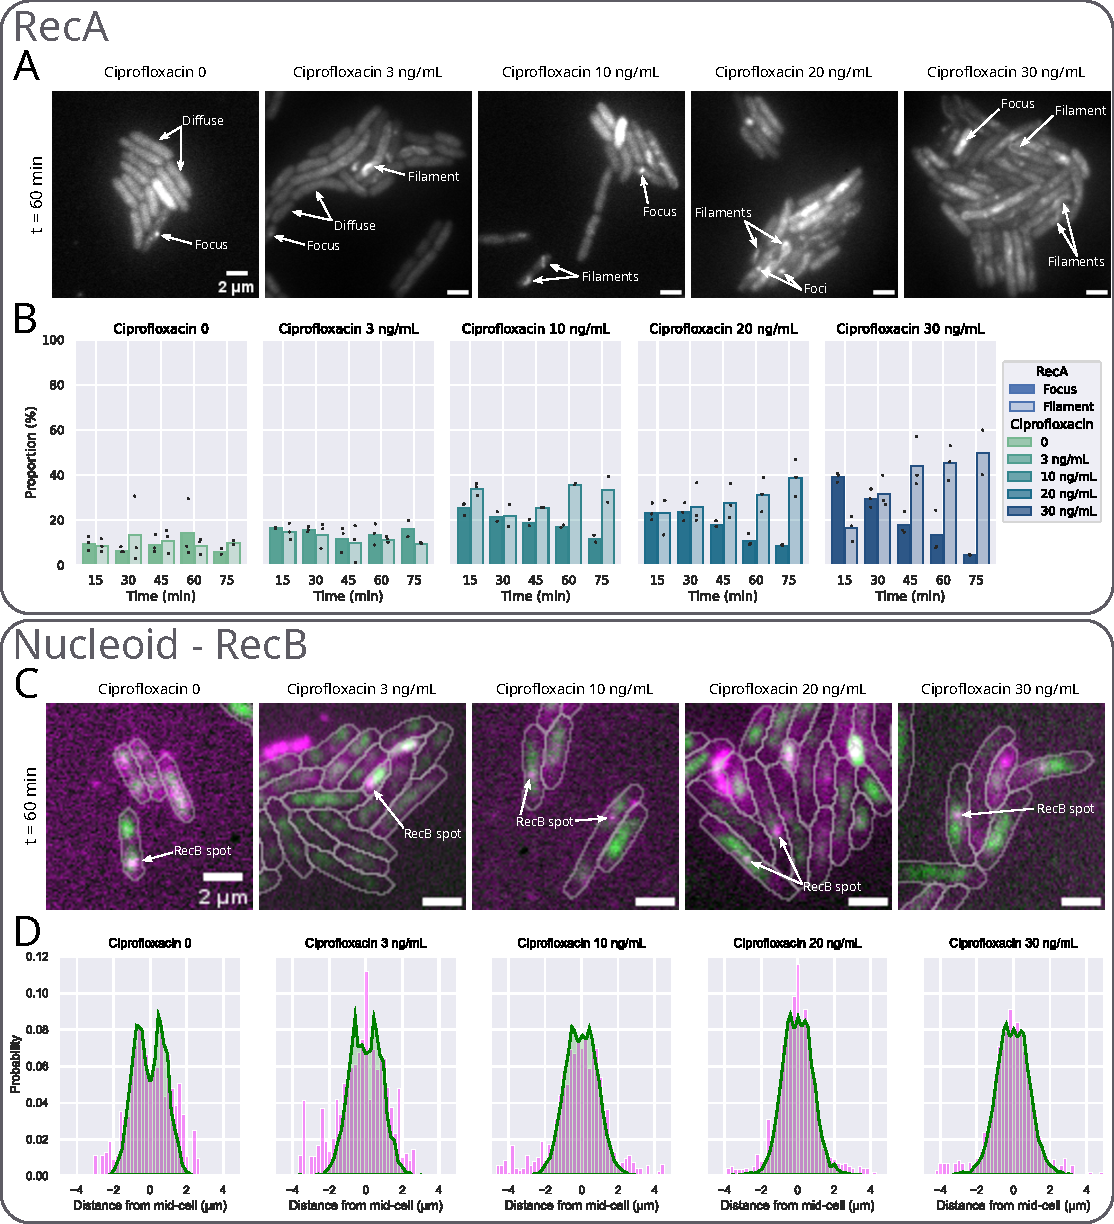
\includegraphics[width=.8\textwidth]{Figures/Fig3_cell_response.pdf}
    \caption{Bacterial cell response to the induction of DSBs by ciprofloxacin. \textbf{(A)} Representative images of cells containing different RecA structures (diffuse fluorescence, foci or filaments) after 60 minutes of exposure to ciprofloxacin. Arrows point to representative examples of each of these structures. \textbf{(B)} Proportion of cells containing RecA foci or filaments. Black dots represent individual datasets, and bars the average between them. \textbf{(C)} Representative images of cells (segmented outline in grey) showing the nucleoid (green) and RecB-associated fluorescence (magenta). RecB spots (indicated by arrows) are located in close proximity to the nucleoid. \textbf{(D)} Overlay of nucleoid density (green area) and position of DNA-bound RecB molecules (magenta bars) along the cell's long axis, for different ciprofloxacin concentrations (0 to 30 ng/mL)}
    \label{Fig:reca_nucleoid}
\end{figure*}

%% We see a strong accumulation of RecA filaments (RecA foci seem to be transient and their number decreases over time)
To paint a more complete picture of the DNA repair process during ciprofloxacin exposure, we imaged the RecA protein fused to the fluorescent protein SYFP2. Figure \ref{Fig:reca_nucleoid}A shows the RecA-associated fluorescence in cells that have been exposed to different concentrations of ciprofloxacin for 60 minutes. In cells that were not exposed to ciprofloxacin, the RecA-associated fluorescence was mostly diffuse, and occasionally formed a bright focus. This is consistent with cells undergoing occasional endogenous DNA damage. As the ciprofloxacin concentration increases, RecA foci became more frequent, as well as filament structures.

To quantify more precisely the occurrence of foci and filaments at the different ciprofloxacin concentrations and durations of exposure, we used a custom-made deep-learning model to automatically classify cells depending on the presence of a focus, a filament, or neither of these structures (Figure \ref{Fig:reca_nucleoid}B, Supp. Figure \ref{SIFig:object_class}). The proportion of cells that contained RecA filaments was initially low under all ciprofloxacin concentrations ($<$20\%). After one hour of exposure the proportion of cells that contained a RecA filament had increased to $\sim$40\% at 20 ng/mL ciprofloxacin, and $\sim$60\% at 30 ng/mL. RecA foci on the other hand seemed to form quickly following ciprofloxacin exposure (present in $\sim$40\% of the cells after 15 min of exposure to 30 ng/mL ciprofloxacin) and come back to endogenous damage level after $\sim$1 hour. Taken together, these results show that RecA foci are transient structures in the repair process that do not accumulate under high DNA damage, whereas RecA filaments do accumulate, presumably when the homologous sequence cannot be found.

%% We imaged nucleoid and RecB in the same experiment
%% Ciprofloxacin exposure causes nucleoid compaction and centring
In \emph{E. coli}, the loading of RecA on DNA triggers the SOS response, which inhibits cell division, leading to cell filamentation. Previous studies have reported that the SOS response also triggers compaction of the bacterial nucleoid.\cite{Odsbu2014} To see if this was the case for breaks induced by ciprofloxacin in our experimental conditions, we stained DNA using the Sytox Green dye. The use of a green dye allowed us to concomittantly image RecB, and to correlate the position of DNA-bound RecB molecules with that of the nucleoid. Figure \ref{Fig:reca_nucleoid}C shows representative images of the nucleoid and DNA-bound RecB after 60 minutes of exposure to different concentrations of ciprofloxacin. In untreated cells, the nucleoid was often observed to be bi-lobed, which is consistent with cells growing exponentially, with high DNA replication activity. Upon exposure to ciprofloxacin, the cells appeared elongated, and the nucleoid was often compacted in the centre of the cell. As a result of the nucleoid compaction, the total fraction of the cell occupied by the nucleoid decreased, from 40\% on average in untreated cells to 31\% in cells exposed to 30 ng/mL of ciprofloxacin for an hour (Supp. Figure \ref{SIFig:nucleoid_compaction}). This compaction was accompanied by a centring of the nucleoid along the cell's long axis. Supp. Figure \ref{SIFig:nucleoid_position} shows that upon increasing exposure to ciprofloxacin (in time and concentration), the cells elongate, and nucleoids were increasingly centred.

%% Nucleoid and RecB position are correlated
%% Interpretation: RecB spot centring is due to nucleoid centring (not obvious: link to RecB recruitment rate, explain it happens after several rounds of DSBs)
As expected, DNA-bound RecB were found in close proximity to the nucleoid (Figure \ref{Fig:reca_nucleoid}C). Figure \ref{Fig:reca_nucleoid}D show the strong overlap between the spatial distribution of DNA-bound RecB spots and the nucleoid density in the cell (Supp. Figure \ref{SIFig:recb_nucleoid_timepoints} shows the same data after different durations of ciprofloxacin exposure). Due to nucleoid compaction and centring, both the nucleoid density and the position of DNA-bound RecB remained within $\sim$2 µm either side of the cell centre, despite the cells having elongated significantly.

%% Overall conclusion on RecA filaments, nucleoid compaction, and correlation of DNA-bound RecB position with nucleoid density
Upon exposure to ciprofloxacin, cells undergoing DSB repair load RecA at the break site, which we were able to detect as bright foci and filaments. At the lower (sub-MIC) ciprofloxacin concentrations, these structures were present in a low proportion of cells (10-20\%). At higher ciprofloxacin concentrations, RecA filaments were present in a large fraction of the cells (up to 40\%), hinting at an accumulation of long-lived RecA filaments unable to find a homologous sequence for repair. RecA loading on DNA also induces the SOS response. As a result, we observed compaction and centring of the bacterial nucleoid. DNA-bound RecB molecules were also found to be centred in elongated cells, consistently with DSBs forming on compacted nucleoids.

% Part 4: Mutants in the repair pathway
\subsection*{RecB dissociation does not depend on RecA loading}

\begin{figure*}[htbp]
    \centering
    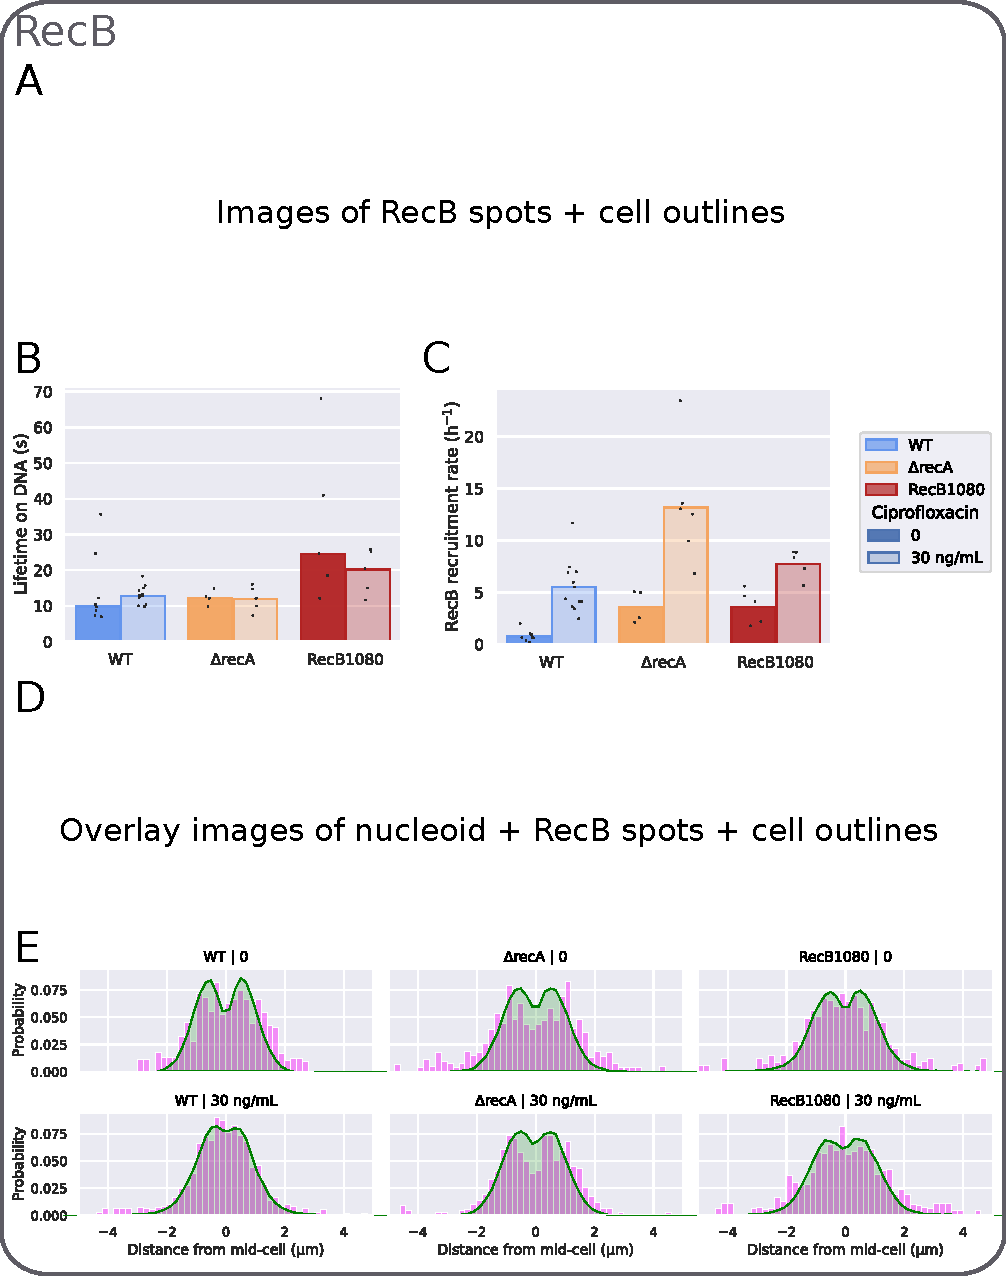
\includegraphics[width=.75\textwidth]{Figures/Fig4_mutants.pdf}
    \caption{RecB binding to DNA in the \dreca\ and \teneighty\ mutant strains in the absence and presence of ciprofloxacin (30 ng/mL). \textbf{(A)} Representative brightfield images of wild-type (WT), \dreca\ and \teneighty\ mutants cells, in the presence and absence of ciprofloxacin (30 ng/mL). \textbf{(B)} Fitted lifetimes of RecB molecules on DNA. Black dots show individual datasets, and bars the median values. \textbf{(C)} Rate of recruitment of RecB to the DNA. Black dots show individual datasets, and bars the median values. \textbf{(D)} Representative overlay images of RecB-associated fluorescence (magenta) and the bacterial nucleoid (green). Segmented cell outline shown in grey. \textbf{(E)} Overlay of nucleoid density (green area) and position of DNA-bound RecB molecules (magenta bars) along the cell's long axis.}
    \label{Fig:mutants}
\end{figure*}

%% Effect of ciprofloxacin exposure on the different mutants
To better understand the factors that contribute to the dissociation of RecB from DNA, we imaged two different mutants (\dreca\ and \teneighty), in the presence and absence of 30 ng/mL ciprofloxacin. Figure \ref{Fig:mutants} shows brightfield images of cells that were not exposed to ciprofloxacin, and cells that were exposed to 30 ng/mL ciprofloxacin for 60 min. Supp. Figure \ref{SIFig:mutants_cell_lengths} shows the average cell length values across conditions and for the different ciprofloxacin exposure durations. As previously observed, wild-type cells show a clear response to exposure to 30 ng/mL ciprofloxacin, where the cell length increases significantly due to induction of the SOS response. In contrast to this, since the \dreca\ mutant is unable to form a RecA filament, it is also unable to induce the SOS response. Cell length therefore remains unchanged, even upon prolonged exposure to 30 ng/mL ciprofloxacin. The \teneighty\ mutant cells were slightly more elongated than wild-type cells in the absence of ciprofloxacin. This matches well with previous indications that this mutant has a higher baseline of SOS induction than wild-type cells in the absence of exogenous DNA damage.\cite{Lepore2023} Upon exposure to ciprofloxacin, the cell length of the \teneighty\ mutant increased, albeit slightly less on average than the wild-type's (Supp. Figure \ref{SIFig:mutants_cell_lengths}). This might be a reflection of \teneighty's inability to load RecA on the DNA, and the use of the alternative RecOR pathway leading to a weaker or delayed SOS response.

%% DNA binding lifetimes
As for the wild-type (WT) strain, we computed histograms of RecB spot lifetimes, and fitted them with a bi-exponential decay model (Supp. Figure \ref{SIFig:mutants_biexp_fits}), from which we extracted the slower rate, corresponding to the dissociation of DNA-bound RecB molecules. The corresponding lifetimes for DNA-bound RecB are shown on Figure \ref{Fig:mutants}B. In the \dreca\ mutant, the DNA-binding lifetime of RecB was similar to the wild-type ($\sim$10 sec). This suggests that RecA loading by RecBCD does not play a role in triggering the dissociation of RecBCD from DNA. Both in the presence and absence of ciprofloxacin, \teneighty\ stayed bound to DNA for longer than wild-type RecB ($\sim$20 sec). This could be due to the inability of \teneighty\ to digest the DNA it unwinds, making dissociation more challenging due to the DNA strands threading through the RecBCD complex.

%% RecB recruitment rate
Estimating the recruitment rate of RecB to the DNA provided additional insight into the dynamics of DSB processing in the \dreca\ and \teneighty\ mutants (Figure \ref{Fig:mutants}C). In the \dreca\ mutant, the rate of recruitment of RecB was increased compared to wild-type cells, both in the presence and absence of ciprofloxacin. As in both cases the rate of DSB formation is expected to be the same between the wild-type and the \dreca\ mutant, we can hypothesise that this higher rate of RecB recruitment to DNA is due to multiple recruitment events on the same original DSB. In the mutant cells, RecBCD processes the DNA, but the generated ssDNA cannot be coated with the RecA protein, and is therefore likely to be degraded by cellular endo- and exonucleases such as SbcCD. Degradation of the ssDNA would lead to a blunting of the DNA end, hence creating a new substrate for RecBCD binding. This deleterious cycle was previously reported to occur in cells lacking the RecA protein, eventually leading to full chromosome degradation\cite{Capaldo1975,Skarstad1993}. In our experiment, it results in multiple recruitments of RecB to DNA for each DSB.

%%% Intermediate recruitment in 1080 compared to WT and ΔrecA, probably resulting from a competition between ssDNA degradation + RecB reloading, and RecA loading + repair
In the \teneighty\ mutant, RecB recruitment is higher than in WT cells, but equivalent (in the absence of ciprofloxacin) or lower (in the presence of 30 ng/mL ciprofloxacin) to the level of RecB recruitment in the \dreca\ mutant (Figure \ref{Fig:mutants}C). Upon DSB recognition, \teneighty\ unwinds DNA without digesting it, and dissociates $\sim$2 times slower than wild-type RecB (Figure \ref{Fig:mutants}B). After RecBCD dissociation, we expect two competing pathways to take place. Either (i) the unwound ssDNA is digested by cellular endo- and exonucleases, creating a new RecBCD substrate; or (ii) RecOR displaces the SSB (Single-Strand DNA-Binding) protein and promotes RecA loading, allowing DNA repair by homologous recombination to proceed. As a result, RecB can be recruited on DNA several times for each DSB (similarly to the \dreca\ mutant), but the cycle of re-recruitment can be broken by the action of RecOR.

%% Compaction of the nucleoid
The differences in induction of the SOS response between the wild-type cells and the mutants resulted in different states of compaction for the bacterial nucleoid (Figure \ref{Fig:mutants}D, Supp. Figure \ref{SIFig:mutants_nucleoid_compaction}). Whereas in the wild-type, exposure to ciprofloxacin triggered compaction and centring of the nucleoid, the inability of the \dreca\ mutant to induce the SOS response resulted in two separate nucleoid regions at the cell poles. Furthermore, several cells appeared to have lower DNA content, consistent with RecBCD degrading large portions of the chromosome. Accordingly, the nucleoid occupied a smaller fraction of the cell in the \dreca\ mutant after exposure to ciprofloxacin (Supp. Figure \ref{SIFig:mutants_nucleoid_compaction}). In the RecB1080 mutant, the nucleoid appeared more disorganised than in wild-type cells, but still underwent compaction at the centre of the cell upon exposure to ciprofloxacin. Notably, the level of compaction of the nucleoid was slightly less important than in wild-type cells (38\% $\pm$ 9 of the cell occupied by the nucleoid after 75 min of exposure to ciprofloxacin, against 32\% $\pm$ 11 in the wild-type). This might again be a reflection of the less efficient RecA loading in this mutant, leading to delayed or weaker SOS response.

%% Colocalisation of RecB with the nucleoid
In all three strains, the localisation of DNA-bound RecB was consistent with that of the bacterial nucleoid, consistent with RecB being recruited to DSBs (Figures \ref{Fig:mutants}D and \ref{Fig:mutants}E). In the \dreca\ mutant, addition of 30 ng/mL ciprofloxacin did not change the spatial distribution of nucleoid density or DNA-bound RecB. This is consistent with \dreca\ cells being unable to induce the SOS response, and therefore not undergoing nucleoid compaction. In the \teneighty\ mutant, both nucleoid density and DNA-bound RecB distributions form a single peak at the cell centre, in the presence and absence of ciprofloxacin. This is consistent with the \teneighty\ mutant having a higher baseline of SOS induction than wild-type cells, as previously reported.\cite{Lepore2023} The slightly broader distribution of nucleoid density and DNA-bound RecB position in the \teneighty\ mutant exposed to ciprofloxacin compared to the wild-type is consistent with the lesser nucleoid compaction observed in this mutant (Figure \ref{SIFig:mutants_nucleoid_compaction}).

\begin{figure*}[htbp]
    \centering
    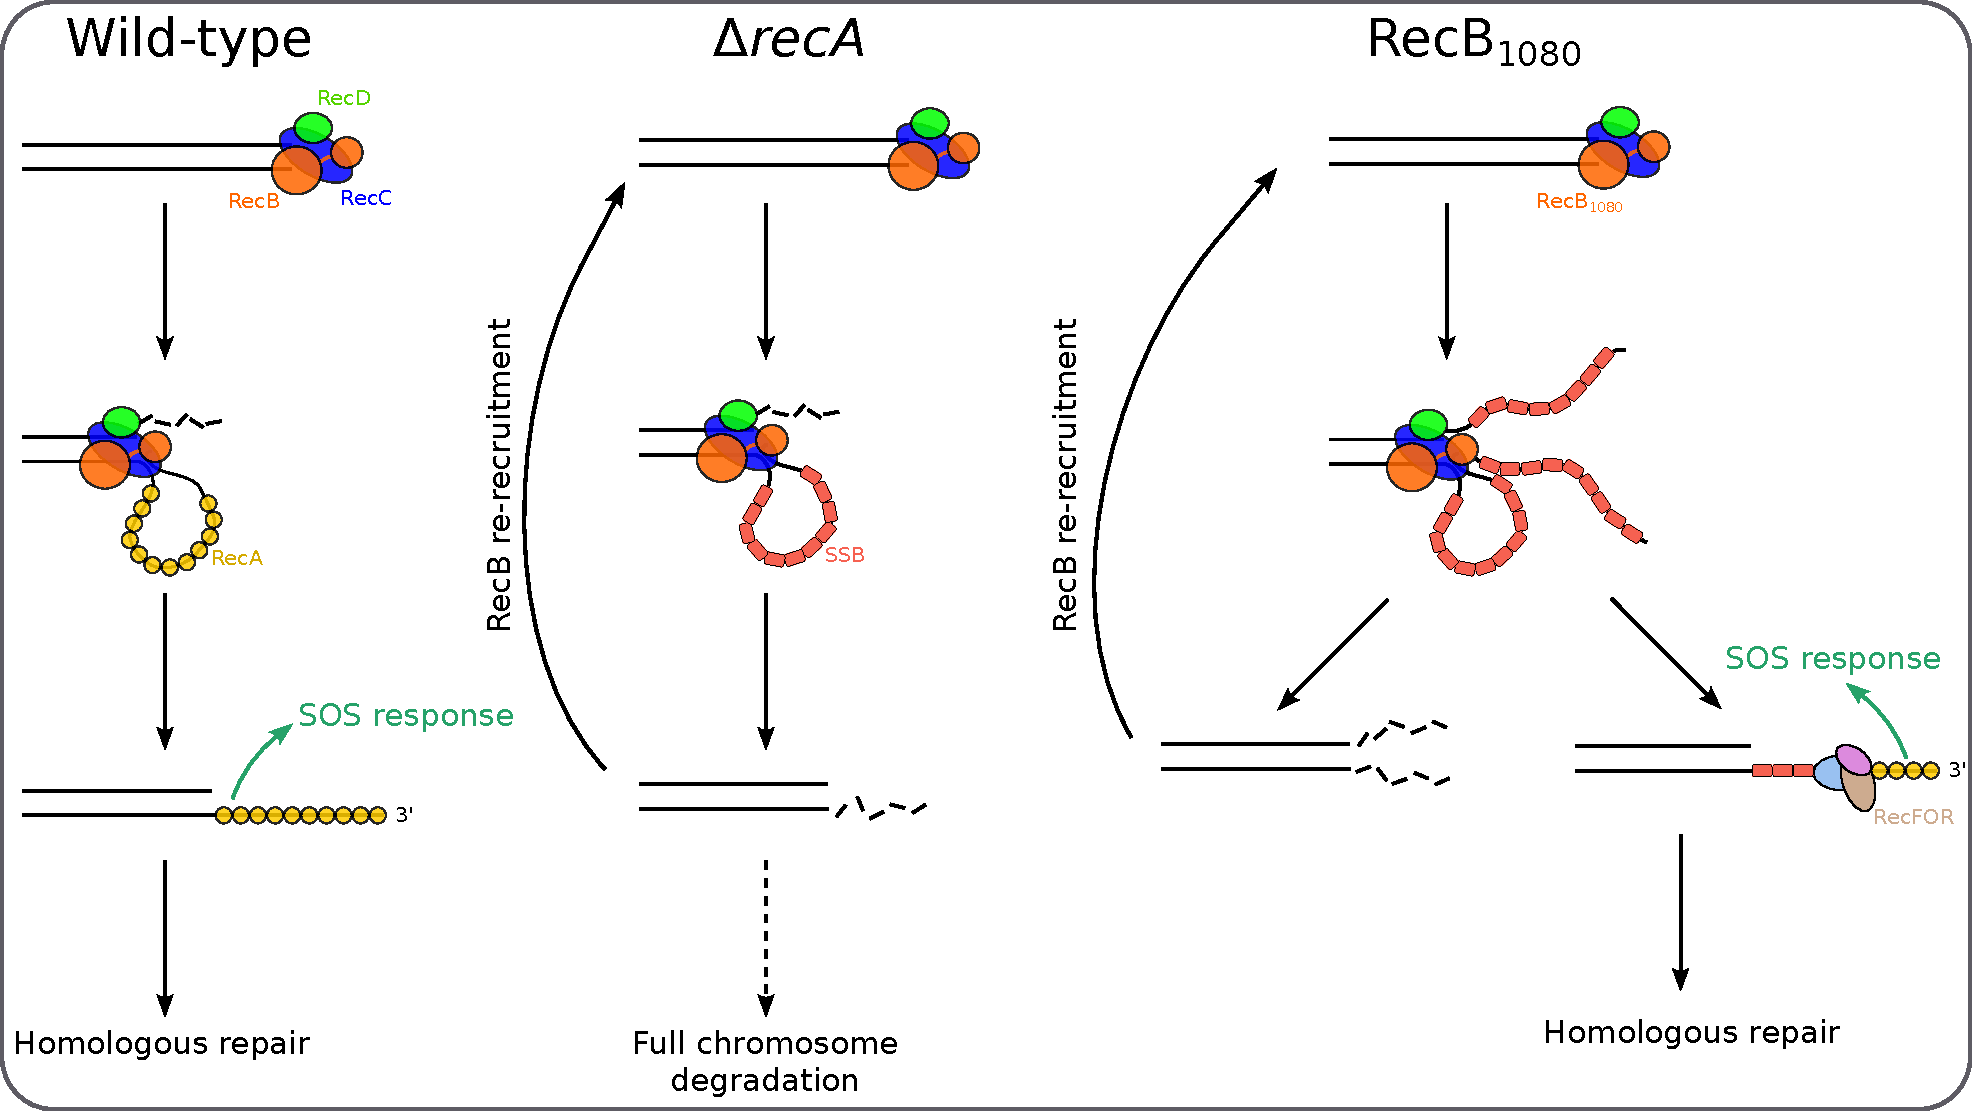
\includegraphics[width=\textwidth]{Figures/Fig_mutants_pathways.pdf}
    \caption{RecBCD recruitment pathways in wild-type \emph{E. coli}, \dreca\ and \teneighty\ mutants. \textbf{(Wild-type)} After DSB recognition, RecBCD degrades DNA until it recognises a Chi-site. It switches activity to create a 3' ssDNA overhang, and promotes RecA loading. The RecA-coated ssDNA can then be used for DNA repair by homologous recombination. \textbf{($\mathbf{\Delta}$reca)} In the absence of RecA, the 3' ssDNA is coated by SSB, and eventually digested by cellular nucleases. Blunting of the DNA end by digestion of the ssDNA creates a new substrate for binding of RecBCD. \textbf{(RecB$\mathbf{_{1080}}$)} Following DSB recognition, \teneighty\ unwinds DNA without digesting it. The unwound ssDNA can either be digested by nucleases, leading to a new blunt dsDNA end and RecBCD re-recruitment; or the RecOR complex displaces SSB to load RecA, allowing DNA repair by homologous recombination to proceed.}
    \label{Fig:pathways}
\end{figure*}

% Different pathways for RecB recruitment to DSBs in the different mutants
Our observations of cell elongation (Figure \ref{Fig:mutants}A), RecB recruitment to DNA (Figure \ref{Fig:mutants}C), and nucleoid position (Figure \ref{Fig:mutants}D) in the different mutant strains have led us to the model of RecB recruitment described in Figure \ref{Fig:pathways}. In wild-type cells, a DSB is recognised by RecBCD, which promotes RecA loading. The RecA filament triggers the SOS response, and is used for homology search and repair. In the \dreca\ mutant, the 3' ssDNA generated by RecBCD is first coated by SSB, and then degraded by cellular nucleases. This leads to blunting of the DNA end, creating a new substrate on which RecBCD can bind. This circle leads to multiple RecBCD recruitments per DSB, and eventually to full chromosome degradation. In the \teneighty\ mutant, RecBCD unwinds DNA without degrading it. After the ssDNA is coated with SSB, two competing pathways take place: either DNA degradation by nucleases leading to DNA-end blunting and re-recruitment of RecBCD, or displacement of SSB by RecOR and loading of RecA, leading to SOS induction and homologous repair.